\chapter{Teknisk beskrivelse}

\section{Databaseabstraktion}

I parallel med Bookie har vi udviklet en databaseabstraktion ved navn \textit{Donkey}. Donkey er bygget oven på JDBC (Java Database Connectivity) og har til formål at muliggøre persistens af datamodeller uden at en udvikler behøver skrive en eneste linje SQL. Dette opnås gennem såkaldt \textit{object-relational mapping} (forkortet \textit{ORM}), hvor et objekt i et objekt-orienteret system–i vores tilfælde Java–automatisk kan konverteres til en mere simpel struktur, som kan gemmes i et databasesystem (\cite{wiki:orm}).

Donkeys grundlæggende byggedele er baserede på Laravels\footnote{\url{http://laravel.com/}} API'er, da disse allerede var en af forfatterne kendte. Konceptuelt låner Donkey begreberne om \textit{Grammars}, \textit{Queries}, samt \textit{Schemas} og benytter disse til at implementere ORM i form af \textit{Models}. En datamodel i Donkey er i sidste ende derfor ikke andet end en klasse, som repræsenterer en tabel i en relationsdatabase, og en række offentlige felter i denne klasse, som repræsenterer tabellens kolonner og datatyperne af disse. Dette er igen relateret til Laravel og dens \textit{Eloquent ORM}\footnote{\url{http://laravel.com/docs/4.2/eloquent}} dog med den forskel, at Donkeys implementation af ORM endnu ikke er nær så fleksibel som Laravels.

Helt konkret består Donkey af følgende klasser:

\begin{multicols}{3}
\begin{itemize}
  \item \texttt{Grammar}
    \begin{itemize}
      \item \texttt{MySqlGrammar}
      \item \texttt{PostgreSqlGrammar}
      \item \texttt{SqliteGrammar}
    \end{itemize}
  \item \texttt{Driver}
  \item \texttt{Row}
  \item \texttt{Database}
  \item \texttt{Query}
  \item \texttt{Schema}
  \item \texttt{Model}
  \item \texttt{ModelQuery}
\end{itemize}
\end{multicols}

Donkey er fra bunden opbygget efter \textit{dependency injection} designmønstret, hvor afhængigheder injiceres i afhængende klasser frem for selv at lade de afhængende klasser finde og instantiere deres afhængigheder (\cite{wiki:di}). Dette designmønster har vi fulgt, da det gav større kontrol over, hvorledes afhængigheder flød igennem systemet. Eftersom \texttt{Grammar}-klassen er en afhængighed i næsten samtlige andre klasser (mere om dette følger), og da \texttt{Grammar} er abstrakt med de konkerete implementationer \texttt{MySqlGrammar}, \texttt{PostgreSqlGrammar}, og \texttt{SqliteGrammar}, ville det have været yderst besværligt at opbygge systemet, hvis ikke denne grundlæggende afhængighed kunne injiceres i de afhængende klasser. Figur \ref{class-diagram:database-abstraction} forsøger at tydeliggøre, hvorledes de forskellige afhængigheder flyder gennem systemet samt hvordan disse injiceres i de afhængende klasser.

\begin{figure}[h]
  \centering
  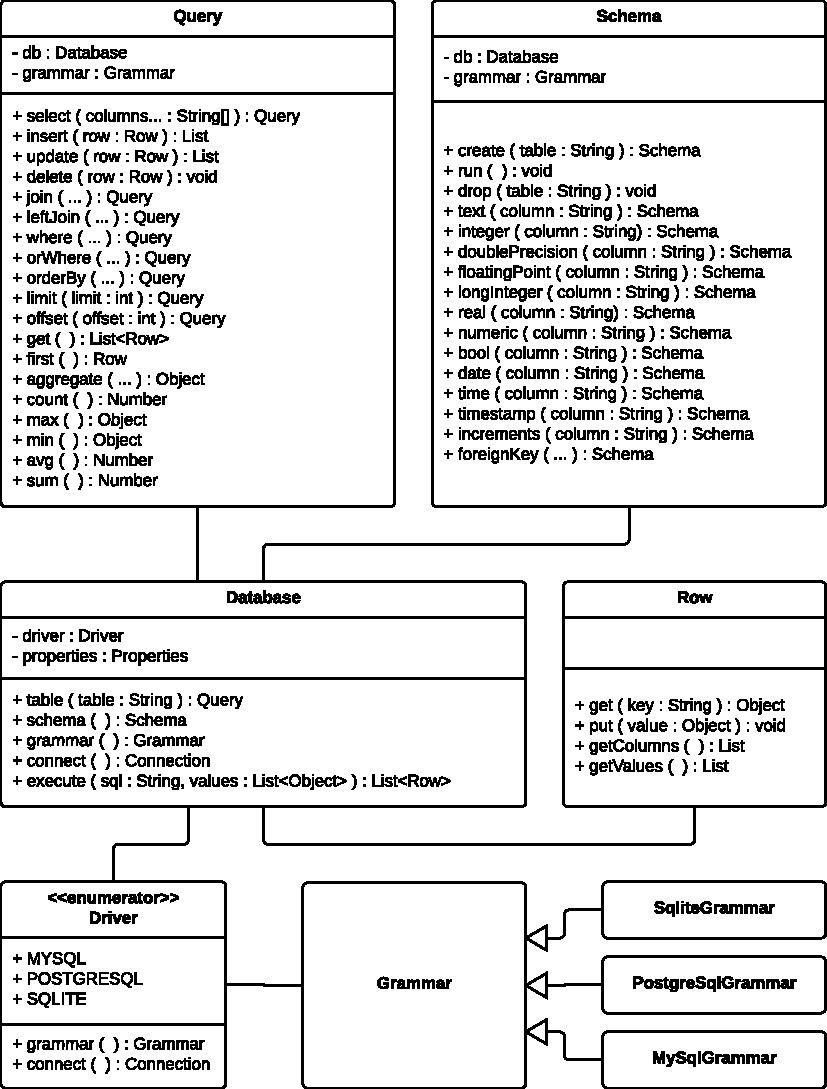
\includegraphics[scale=0.75]{database-abstraction.pdf}
  \caption{Lettere forsimplet klassediagram over databaseabstraktionen, ORM ekskluderet.}
  \label{class-diagram:database-abstraction}
\end{figure}

De næste sektioner vil gennemgå hver klasse i det niveau af detalje, som måtte være sig passende for den enkelte klasse.

\subsection{Row}

\texttt{Row}-klassen er en subklasse af \texttt{LinkedHashMap} og beskriver en datastruktur, som benyttes til at opbevare databaserækker. Den er fundamental for resten af systemet, idet den er bindeledet mellem Donkeys klasser og JDBCs \texttt{ResultSet}\footnote{\url{https://docs.oracle.com/javase/8/docs/api/java/sql/ResultSet.html}}-strukturer, som bruges til at opbevare tabeller af data resulterende fra databaseforespørgsler.

\subsection{Grammar}

\subsection{Driver}

\subsection{Database}

\subsection{Query}

\subsection{Schema}

\subsection{Model}

\subsection{ModelQuery}

\section{Databasedesign}